% \documentclass[9pt,a4paper,twocolumn,landscape,oneside]{amsart}
\documentclass[8pt,a4paper,landscape,oneside]{amsart}
\usepackage{amsmath, amsthm, amssymb, amsfonts}
\usepackage[T1]{fontenc}
\usepackage[utf8]{inputenc}
\usepackage{booktabs}
\usepackage{fancyhdr}
\usepackage{float}
\usepackage{fullpage}
%\usepackage{geometry}
\usepackage[landscape]{geometry}
% \usepackage{listings}
\usepackage{caption, subcaption}
\usepackage[scaled]{beramono}
\usepackage{color,graphicx,overpic}
\usepackage{titling}
\usepackage{datetime}
\usepackage{multicol}
\usepackage{calc}
\usepackage{ifthen}
\usepackage{hyperref}
\usepackage{environ}
\usepackage{tabularx}
\usepackage[dvipsnames]{xcolor}


% Minted (For code stuff)
\usepackage{minted}
\newcommand{\code}[1]{\inputminted[fontsize=\footnotesize]{c}{#1}}

% This sets the margins to .5cm
\geometry{top=0pt,left=.3cm,right=.3cm,bottom=1cm}

\setlength{\headheight}{15.2pt}
\renewcommand{\headrulewidth}{0.4pt}
\renewcommand{\footrulewidth}{0.4pt}

% Turn off header and footer
% \pagestyle{empty}

% Redefine section commands to use less space
\makeatletter
\renewcommand{\section}{\@startsection{section}{1}{0mm}%
                                {-1ex plus -.5ex minus -.2ex}%
                                {0.5ex plus .2ex}%x
                                {\normalfont\large\bfseries}}
\renewcommand{\subsection}{\@startsection{subsection}{2}{0mm}%
                                {-1explus -.5ex minus -.2ex}%
                                {0.5ex plus .2ex}%
                                {\normalfont\normalsize\bfseries}}
\renewcommand{\subsubsection}{\@startsection{subsubsection}{3}{0mm}%
                                {-1ex plus -.5ex minus -.2ex}%
                                {1ex plus .2ex}%
                                {\normalfont\small\bfseries}}
\makeatother


% Don't print section numbers
\setcounter{secnumdepth}{0}


\setlength{\parindent}{0pt}
\setlength{\parskip}{0pt plus 0.5ex}

\newcommand{\subtitle}[1]{%
  \posttitle{%
    \par\end{center}
    \begin{center}\large#1\end{center}
    \vskip0.5em}%
}

% Header/Footer
% \geometry{includeheadfoot}
% \fancyhf{}
\pagestyle{fancy}
\lhead{HSR}
\rhead{Silvan Adrian\quad\thepage}
\cfoot{}

% Title/Author
\title{WED2 Cheat Sheet}
\subtitle{}
\date{\ddmmyyyydate{\today{}}}

% Output Verbosity
\newif\ifverbose
\verbosetrue
% \verbosefalse

% Some list helpers from graph theory
\newcounter{temp}
\newcounter{ilist_counter}
\newcounter{iilist_counter}

\newenvironment{ilist}{
  \begin{list}{{\bf \arabic{ilist_counter}}}{
      \usecounter{ilist_counter}
      \addtolength{\labelsep}{.6ex}
      \addtolength{\itemsep}{1ex}
      \setlength{\leftmargin}{1.4em}}
    %   \setcounter{ilist_counter}{\value{temp}}
}{
%   \setcounter{temp}{\value{ilist_counter}}  
  \end{list}
}

\newenvironment{iilist}{
  \begin{list}{{\bf \alph{iilist_counter}}}{
      \usecounter{iilist_counter}
      \addtolength{\labelsep}{.6ex}
      \addtolength{\itemsep}{.5ex}
      \setlength{\leftmargin}{1.7em}}
}{
  \end{list}
}

\newenvironment{iblist}{
  \begin{list}{{\bf $\bullet$}}{
      \addtolength{\labelsep}{.6ex}
      \addtolength{\itemsep}{.5ex}
      \setlength{\leftmargin}{1.7em}}
}{
  \end{list}
}

% Theorems and solutions
\theoremstyle{plain}
\newtheorem{theorem}{Theorem}
\newtheorem*{theorem*}{Theorem}
\newtheorem{corollary}[theorem]{Corollary}
\newtheorem*{corollary*}{Corollary}
\newtheorem{lemma}[theorem]{Lemma}
\newtheorem*{lemma*}{Lemma}
\newtheorem{proposition}[theorem]{Proposition}
\newtheorem*{proposition*}{Proposition}
\newtheorem{conjecture}[theorem]{Conjecture}
\newtheorem*{conjecture*}{Conjecture}
\newtheorem*{solution}{Solution}

\theoremstyle{definition}
\newtheorem{definition}[theorem]{Definition}
\newtheorem*{definition*}{Definition}
\newtheorem{example}[theorem]{Example}
\newtheorem*{example*}{Example}
\newtheorem{problem}[theorem]{Problem}
\newtheorem*{problem*}{Problem}

\theoremstyle{remark}
\newtheorem{remark}{Remark}
\newtheorem*{remark*}{Remark}

% For writing vectors
\let\oldhat\hat
\let\oldvec\vec
\renewcommand{\vec}[1]{\oldvec{\mathbf{#1}}}
\newcommand{\vecb}[1]{\mathbf{#1}}
\renewcommand{\hat}[1]{\oldhat{\mathbf{#1}}}

\newcommand{\cvect}[2]{ \begin{pmatrix} #1 \\ #2 \end{pmatrix} }
\newcommand{\ctvect}[3]{ \begin{pmatrix} #1 \\ #2 \\ #3 \end{pmatrix} }
\newcommand{\vect}[2]{ \langle #1 , #2 \rangle }
\newcommand{\tvect}[3]{ \langle #1 , #2 , #3 \rangle }
\newcommand{\qvect}[4]{ \langle #1 , #2 , #3 \rangle }

% For equations
\NewEnviron{formula}{
    \abovedisplayshortskip=0pt
    \belowdisplayshortskip=0pt
    \abovedisplayskip=0pt
    \belowdisplayskip=0pt
    \begin{align*}
        \BODY
    \end{align*}
}
\newcommand{\eqn}[1]{\begin{formula} #1 \end{formula}}
% The actual document

\newcounter{line}
\newcolumntype{C}{>{\ttfamily\arraybackslash}l}
\newcolumntype{E}{>{\ttfamily\arraybackslash}c}
\newcolumntype{R}{>{\ttfamily\arraybackslash}r}
\newcolumntype{b}{>{\bfseries\arraybackslash}l}
\newenvironment{tabularlc}[1]{
\setcounter{line}{0}
\begin{tabular}{#1}
}{
\end{tabular}
}
\newenvironment{ldesc}{
\begin{tabularlc}{lC}
}{
\end{tabularlc}
}
\newenvironment{Ldesc}{
\begin{ldesc}
\hline
}{
\\\hline
\end{ldesc}
}
\newcommand{\C}{\texttt}
\newcommand{\B}{\textbf}
\newcommand{\I}{\textit}
\newcommand{\CI}[1]{\texttt{\textit{#1}}}
\newcommand{\N}{\textnormal}
\newcommand{\T}[1]{\hphantom{\I{#1}}}
\newcommand{\D}[1]{\hphantom{#1}}
\newcommand{\lditem}[2]{
	#1 & #2 \\
}
\newcommand{\li}[1][]{%
\stepcounter{line}%
\ifnum\theline>1 \\\fi%
#1 &
}
\newcommand{\lI}[1][]{%
\stepcounter{line}%
\ifnum\theline>1 \\[1ex]\fi%
#1 &
}
\newcommand{\Li}[1][]{%
\stepcounter{line}%
\ifnum\theline>1 \\\hline\fi%
#1 &
}
\newcommand{\LI}[1][]{%
\stepcounter{line}%
\ifnum\theline>1 \\[1ex]\fi%
#1 &
}
\newcommand{\s}{\hphantom{A}}
\newcommand{\comm}[1]{\textcolor{gray}{#1}}
\newcommand{\commi}[1]{\textit{\comm{#1}}}
\newcommand{\la}{\textbackslash}
\newcommand{\mtype}[1]{\multicolumn{2}{@{}C}{#1}}
\newcommand{\longtype}[1]{\multicolumn{3}{@{}C}{#1}}
\newcommand{\Longtype}[1]{\multicolumn{4}{@{}C}{#1}}
\newcommand{\longcall}[1]{\multicolumn{3}{@{}R@{\s$\equiv$\s}}{#1}}
\newcommand{\F}{\I{f}}
\newcommand{\X}{\I{x}}
\newcommand{\Y}{\I{y}}
\newcommand{\Z}{\I{z}}
\newcommand{\W}{\I{w}}
\newcommand{\XS}{\I{xs}}
\begin{document}
%\maketitle
\thispagestyle{fancy}
\raggedright
\footnotesize
\raggedcolumns
\begin{multicols*}{4}
\setlength{\premulticols}{1pt}
\setlength{\postmulticols}{1pt}
\setlength{\multicolsep}{1pt}
\setlength{\columnsep}{2pt}
\tiny
\subsubsection{Begriffe}
\textbf{\color{ForestGreen}AJAX:} 
Asynchronous JavaScript and XML.
\textbf{\color{ForestGreen}AMD  (Asynchronous  Module  Definition):} 
Ist  eine  JS  Spezifikation,  welche  es  erlaubt  Module 
und  ihre  Abhängigkeiten  asynchron  zu  laden.  Vorteile:  Webseiten  Performance  Improvement, 
erlaubt  es  Abhängigkeiten 
zu  definieren,  welche  vor  dem  eigentlichen  Modul  geladen  werden sollen. 
\textbf{\color{ForestGreen}Card  Sorting:}
Methode  zur  Bestimmung  verständlicher  Navigationshierarchien.  Ausgeführt  von 
der zukünftigen Benutzergruppe.
\textbf{\color{ForestGreen}Closures:} 
Inner,  nested  anonymous  function,  welche  Zugriff  auf  die  äusseren  Funktionsvariablen hat. 
\textbf{\color{ForestGreen}Context:} 
Repräsentiert den Objekt eigenen Memory Bereich (this).
\textbf{\color{ForestGreen}CSS-Pixel:} 
Die  «Device-Pixel-Ratio»  definiert  das  Verhältnis  zwischen  Device-Pixel  und  CSS-Pixel 
\textbf{\color{ForestGreen}Direktiven  (AngularJS):}  Mächtiges  Konzept  
zur  Erweiterung  von  HTML  durch  Attribute  und 
Elemente.
\textbf{\color{ForestGreen}Event driven  \&  NonBlocking:}
Während  ein  Request  auf  seine  Antwort  wartet,  darf  in  dieser 
Zeit der Node Prozess nicht blockiert werden. Wenn ein Request fertig bearbeitet wurde, wird ein 
Event generiert und der dazugehörige Callback ausgeführt.
\textbf{\color{ForestGreen}Graceful Degradation:} Alle Features werden genutzt, allen dies nicht unterstützen eine 
Alternative bieten (günstigere Entwicklung, teurere Wartung).
 \textbf{\color{ForestGreen}HATEOAS:} 
Hypermedia  as  the  Engine  of  Application  State. 
D.h.  Response  liefert  Ressourcen, die man als nächstes 
ansprechen kann und was man damit tun kann.
\textbf{\color{ForestGreen}Idempotenz:} 
Request seriell mehrfach ausgeführt -> immer gleiches Ergebnis.
\textbf{\color{ForestGreen}Idiom:} 
Beschreibt  ein  einfaches  Feature  was  nativ  nicht  ein  eine  Technologie/Prog  lang.  integriert 
ist.
\textbf{\color{ForestGreen}Middleware:}
Express Plugin Erweiterungen und Handler in der Verarbeitung von Requests.
\textbf{\color{ForestGreen}Modernizr:} Responsive Design Plugin, dass aufgrund von unterstützten Browser 
Features CSS Classes den HTML Tags hinzufügt.
\textbf{\color{ForestGreen}MVVM:} Model View ViewModel  Pattern  (sehr  ähnlich  dem  MVC  Pattern).  
Viewmodel  ist  ein 
“Controler”, der nur States und Operations von 
einer 
View handelt.
\textbf{\color{ForestGreen}Polyfill:} Ein  Polyfill  ist  ein,  oft  in  Javascript  geschriebender,  Code
Baustein,  der  in  älteren 
Browsern eine neuere, von 
diesem nicht unterstützten Funktion
mittels eines Workarounds nach-
rüsten soll. 
\textbf{\color{ForestGreen}Progressive Enhancement:}
Start mit Grundfunktionalität, wenn unterstützt zusätzliche Features 
bieten (teure Entwicklung, billigere Wartung). 
\textbf{\color{ForestGreen}Server  Push:} 
Server  Push  wurde  in  der  Vergangenheit  mit  Polling  (Client  geht  in  bestimmten 
Intervall immer wieder abfragen) umgesetzt. Seit einiger Zeit gibt es Websockets dafür. 
\textbf{\color{ForestGreen}Socket.io:} Verbreitetste WebSocket Library, muss 
auch in der Client App eingebunden werden. 
Kann Broadcast Nachricht an alle Clients senden und bietet Fallback auf Polling.
\textbf{\color{ForestGreen}Token:} 
Problem:  Mit  REST  will  man  Stateless
sein,  ist  man  aber  mit  Sessions  nicht.  Token 
ersetzt  Session.  Idee:  Bei  jeder  Anfrage  wird  ein  Token  generiert  +  mit  gegeben 
enthält  alle Infos zur Autorisierung. Im Token ist eine einmalige zufällige Nummer gespeichert. In der
 Datenbank liegt die Information zu wem das Token gehört. 
\textbf{\color{ForestGreen}WebSockets:} WebSockets  ermöglichen  das  Öffnen  eines  
Channels,  der  bidirektional  benutzt 
werden kann. 
\textbf{\color{ForestGreen}Shared Element Transition:} Bei Android eine 
Actitivity, die sich aus mehreren Fragments zusammensetzte und die Übergänge für 
die Fragments macht ,dabei soll nicht immer eine volle Animation gezeigt werden (schnellere 
Übergänge).


\subsection{Design}
\begin{multicols}{2}
\subsubsection{Cognitive Walktrough / Usability Testing}
\tiny Ist eine je Methode zur Identifikation von Usability Problemen. Cognitive 
Walktrough wird durchgeführt von 3 oder mehr Experten und Usability Testing 
von 3 oder mehr zukünftigen Nutzer. Für Usability Testing braucht es noch kein 
lauffähiges System, Screenshots reichen. Grösste Herausforderung bei Usability 
Testing ist die Erstellung guter Aufgaben, bei welchen echte Benutzerziele getestet 
werden ohne, dass Keywords verraten werden.
\subsubsection{User Centered Design}
Elemente der User Experience: Oberfläche (Aufmerksamkeiten, 
Erkennung von Bekanntem), Raster (Responsive Design), Struktur (Usability), 
Umfang, Strategie.
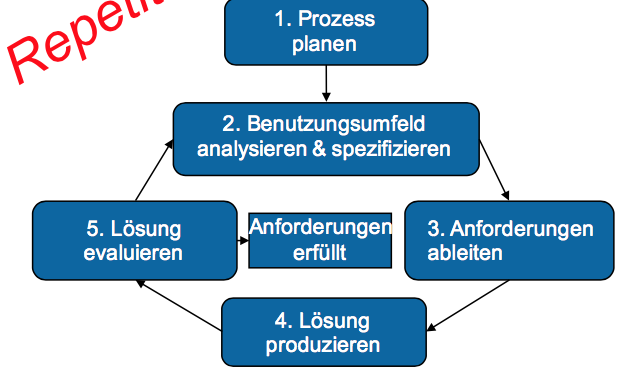
\includegraphics[width=0.12\textwidth]{images/ucd}
\subsubsection{Responsive layout}
Webseiten mit responsivem Layout sind sowohl fluid, als auch adaptiv.
 \textbf{Fluid:} Zusätzlicher Platz wird durch verbreitern der Elemente ausgefüllt. 
\textbf{Adaptiv:} Zusätzlicher Platz wird durch Umordnen und zusätzliche Elemente (oder Spalten) ausgefüllt
\end{multicols}
\begin{multicols}{5}
  \textbf{Mast./Det. Pattern}
  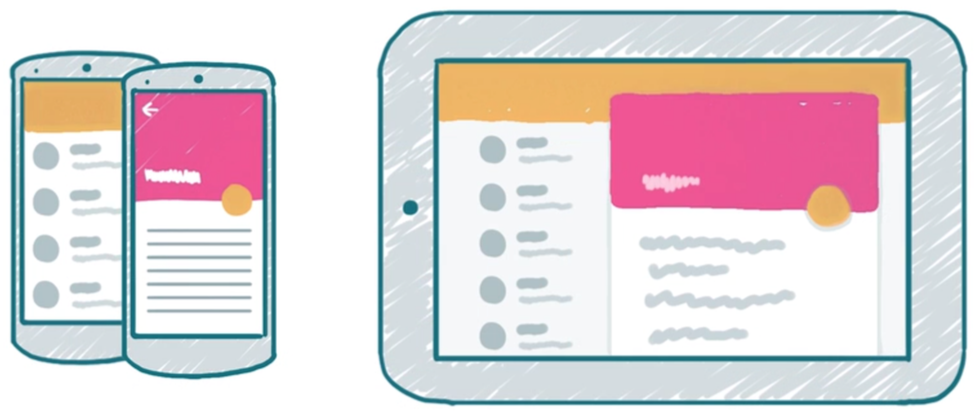
\includegraphics[width=0.045\textwidth]{images/master}
  
  \textbf{Off-Screen Menu (Mob) und On-Screen Menu (Tab./Des.)}
  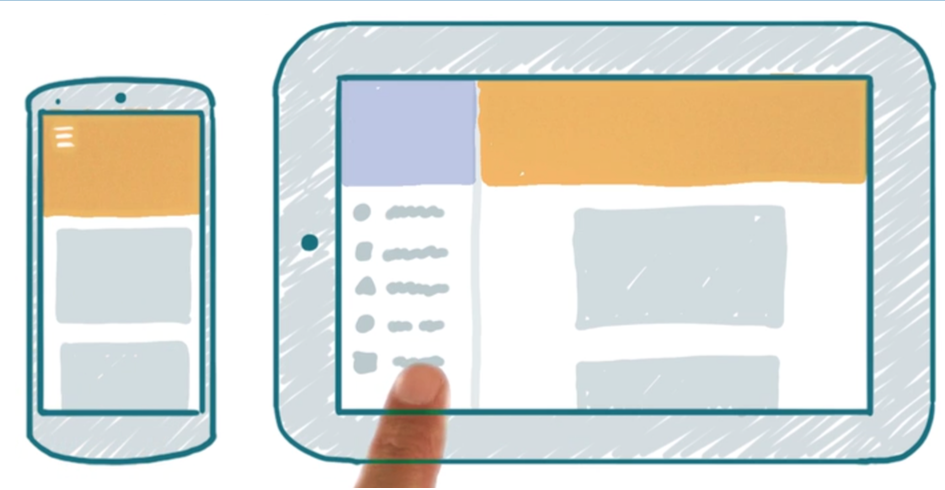
\includegraphics[width=0.045\textwidth]{images/offscreen}
  
  \textbf{Maximale Breite/Rand}
    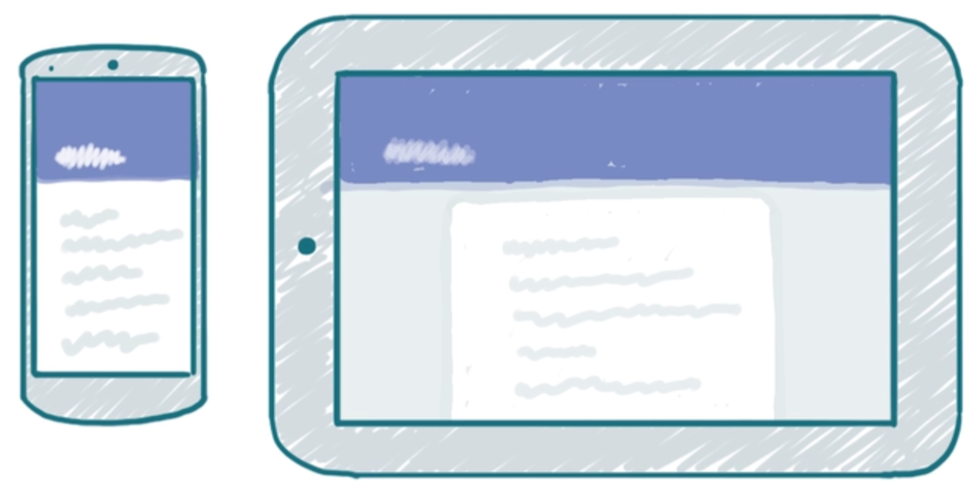
\includegraphics[width=0.045\textwidth]{images/maxbreite}
    
  \textbf{“Reflow” Eine Spalte (Mob.) und viele Spalten (Tab./Des.)}
   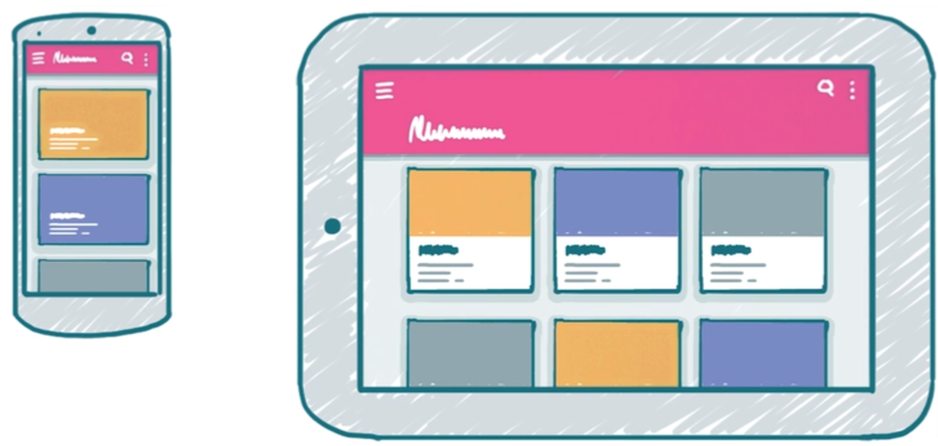
\includegraphics[width=0.045\textwidth]{images/reflow}
   
  \textbf{Sidebar / SidePic für Landscape Ansicht}
  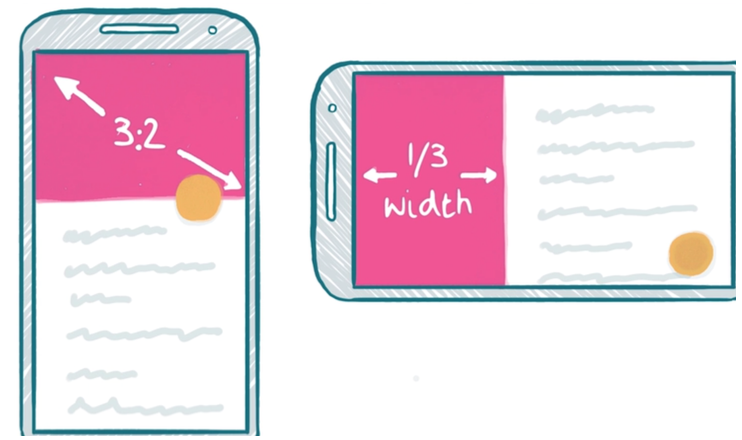
\includegraphics[width=0.045\textwidth]{images/landscape}
\end{multicols}
\begin{multicols}{2}
  Scenario: (Vorgeschichte, Ziel, Startpunkt, Benutzerprofil).
  Nach jed. Schritt (Sichtbarkeit (weg zum Ziel), 
  Affordance (wie bedienen), Feedback (geklappt?))
  \vfill
  \columnbreak
  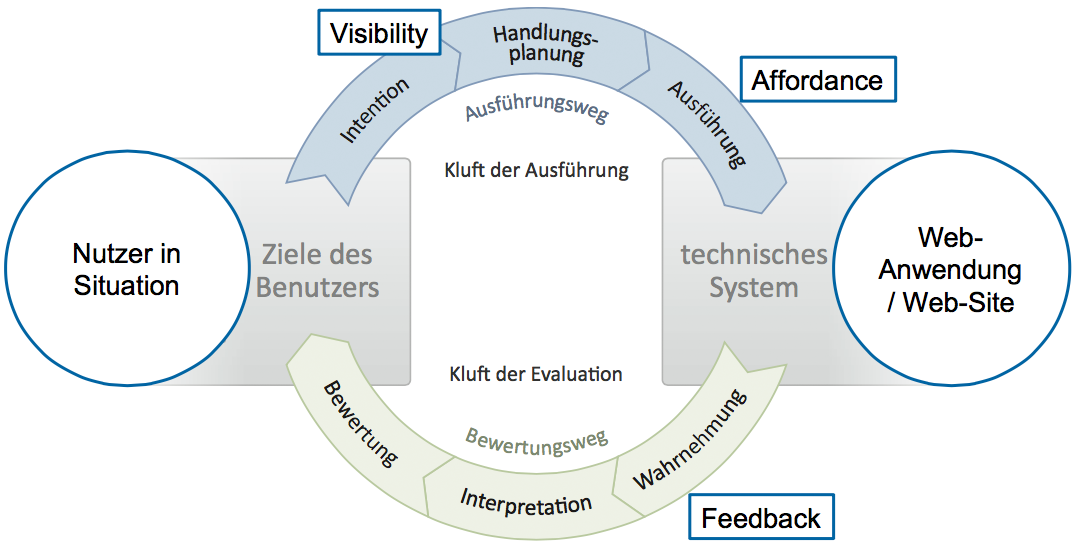
\includegraphics[width=0.11\textwidth]{images/stone}
\end{multicols}


\subsubsection{Flex}
 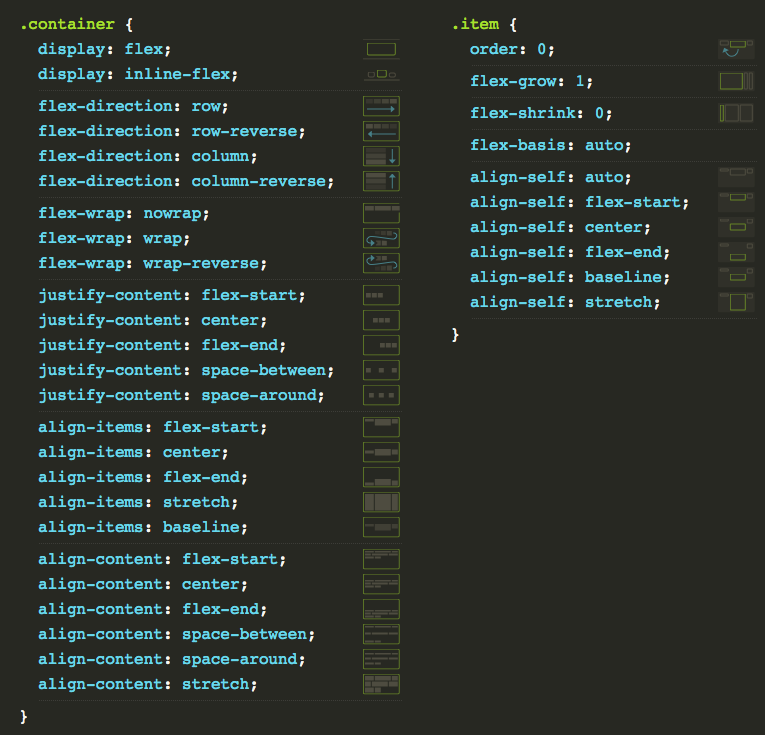
\includegraphics[width=0.25\textwidth]{images/flexbox}
 \begin{minted}[frame=none,framesep=1mm,fontsize=\tiny]{css}
*{ box-sizing: border-box; padding: 0px; margin: 0px;}
#containerMain{ display: flex; flex-flow: column; height: 100%;}
#container{display: flex;flex-flow: row;padding: 0px;}
div{ flex: 1; border: 1px solid blue;}
.content{ flex : 3 1 50%; overflow-y: auto;}
.aside{ flex: 0 0 auto; }
.header, .footer { flex: 0 0 auto;}
#root{ height: 100vh; }
/* Three values: flex-grow | flex-shrink | flex-basis */
flex: 2 2 10%;
\end{minted}
 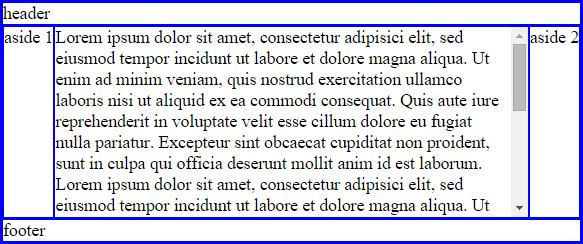
\includegraphics[width=0.25\textwidth]{images/borderlayout}
\subsubsection{Media Queries}
Bevorzugt die Grössen immer in “em” angeben, 
dann dann die Default-Font Size im Browser berücksichtigt wird.
 \begin{minted}[frame=none,framesep=1mm,fontsize=\tiny]{css}
@media only screen and (max|min|-width: 500px), only ...
@media only screen and (max|min|-height: 500px)
@media only screen and (orientation: landscape)
@media only screen and (min-device-pixel-ratio: 2) and (min-width: 1300px)
\end{minted}
 \begin{minted}[frame=none,framesep=1mm,fontsize=\tiny]{html}
<!-- responsive images -->
<picture>
<source media="(min-width: 650px)" srcset="images/kitten-large.png">
<source media="(min-width: 465px)" srcset="images/kitten-medium.png">
<!-- img tag for browsers that do not support picture element -->
<img src="images/kitten-small.png" alt="a cute kitten">
</picture>
<img src="image-src.png" srcset="image-1x.png 1x, image-2x.png 2x,
 image-3x.png 3x, image-4x.png 4x">
\end{minted}

\subsubsection{Viewport}
Mobile Browser erzeugen einen virtuellen Viewport und Zoomen auf eine «sinnvolle» Grösse. 
Der «meta»-Tag 
verlangt das der virtuelle Viewport gleich gross ist wie die «ideale» Grösse vom Gerät
 \begin{minted}[frame=none,framesep=1mm,fontsize=\tiny]{html}
<meta name="viewport" content="width=device-width, initial-scale=1.0, 
user-scalable=no">
<!-- initial-scale: anfaenglichen Zoomgrad 1.0 -> 1:1, 2.0 waere eine 2 fache 
Vergroesserung -->
<!-- user-scalable: Nutzer kann zoomen yes/no -->
<!-- minimum/maximum-scale: Zoom einschraenken -->
\end{minted}

\subsubsection{SASS/SCSS}
Präprozessor für CSS Code. Ermöglicht effizienteren + wartbareren Code zu schreiben, 
ermöglicht ohne Copy \& Paste zu arbeiten und Modularisierung. Kennt Variablen , 
Referenzen (\&), Placeholder (\%), Steuerzeichen (@, wi e @if), Interpolation/Einsetzen. 
Erlaubt Definitionen zu 
“nesten”, CSS Definitionen auf mehrere Files zu verteilen. 
Mixins können auch Parameter haben
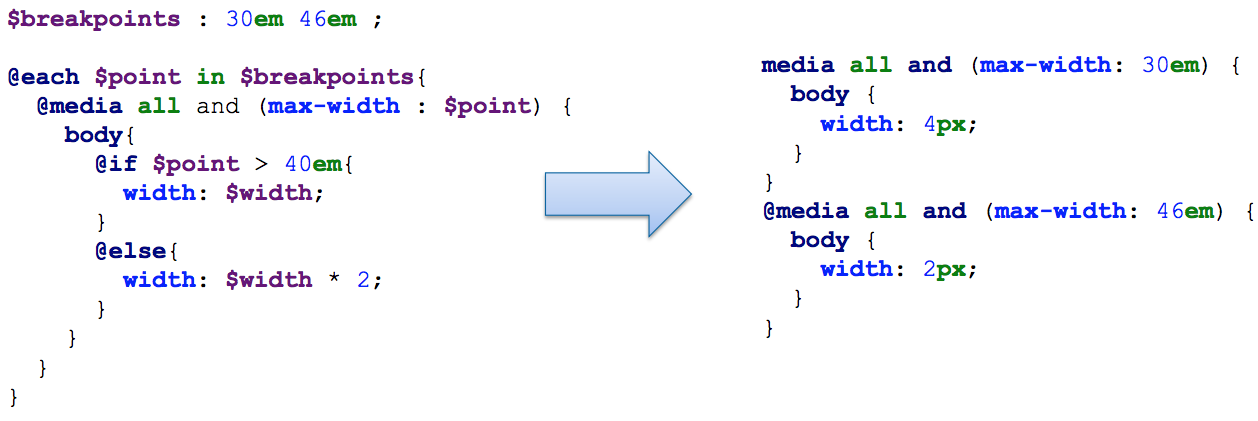
\includegraphics[width=0.25\textwidth]{images/scssloop}
 \begin{minted}[frame=none,framesep=1mm,fontsize=\tiny]{scss}
@mixin shadow( $x ) { //auch ohne uebergabe
  border: $x; //via @Inlcude aufrufen
} //@Extend an bestehende Class anhaengen
//%fuegt es in bestehende ein
$wk: -webkit-;
.rounded-box {
  #{$wk}border-radius: 4px;
}
@Import 'FileXY';
 \end{minted}
\subsubsection{JS OO}
\subsubsection{Scope / Context}
“Abnormal Context Behavior” (Beispielcode rechts ->) entsteht, 
wenn mittels “this.XY” Variablen oder Funktionen innerhalb einer Object 
Funktion definiert werden, ohne dass mit “var self = this;” das “this” erst auf das Objekt 
gebunden wird und das Objekt ohne “new” instanziert wurde. 
In einem solchen Fall, werden die Variablen und Funktionen nämlich auf dem globalen Context gespeichert.
 \begin{minted}[frame=none,framesep=1mm,fontsize=\tiny]{javascript}
function House (color) { 
  this.facadeColor = color; 
  this.paint = function(newColor) {
this.facadeColor = newColor;
}; }
var whiteHouse = new House("white"); 
whiteHouse.paint("beige");
var whiteHouse = House("white"); // auf globalem Context, da ohne new
//abnormal Context umgehen oder auf Object binden
function House (color) {
var self = this; //auf Scope speichern
  self.facadeColor = color; 
  self.paint = function(newColor) {
  self.facadeColor = newColor;
}; }
var whiteHouse = new House("white"); 
whiteHouse.paint("beige");
var paintWhiteHouse = whiteHouse.paint; 
paintWhiteHouse("red");
//Closure
function myFunction(arg){
  var inner = 5;
  var getInner = function() {
      return arg || inner;
  };
  return getInner;
}
var getInnerPtr = myFunction(); 
// returns the function pointer to getInner 
var innerValue = getInnerPtr(); // execute getInner function
\end{minted}

\subsubsection{OOP}
\textbf{\color{MidnightBlue}Constructor Pattern:} Ermöglicht das
aufzwingen von “new”, selbst wenn man den
Konstruktor wie eine Funktion
aufruft.
 \begin{minted}[frame=none,framesep=1mm,fontsize=\tiny]{javascript}
var ConstructorName = (function() {
'use strict';
function ConstructorName(arg1, arg2) {
// enforces new
if (!(this instanceof ConstructorName)) { return new ConstructorName();
}
// constructor body }
ConstructorName.prototype.someMethod = function(arg) { // method body
}
return ConstructorName;
}());
\end{minted}
\textbf{\color{MidnightBlue}Module Pattern:} Lokale Variablen
sind völlig vom global scope abgeschirmt und deren Lebenszeit ist auf
die Module’s closure begrenzt.
Module schützen namespaceing,
public und private Variablen.
 \begin{minted}[frame=none,framesep=1mm,fontsize=\tiny]{javascript}
var moduleName = (function() {
var privateVar;
function privateMember(arg1, arg2) {
// method body }
return {
member: function (arg1, arg2) {
// public method body; contains implementation and uses private members... }
};
}()); // use it with moduleName.member()
\end{minted}

\textbf{\color{MidnightBlue}Revealing module pattern:} Modularisierung des Codes, Bildet
abgeschlossenen Namespace durch
Function Scope. Abhängigkeiten müssen von Hand definiert
werden. Für grosse Applikationen ungeeignet.
 \begin{minted}[frame=none,framesep=1mm,fontsize=\tiny]{javascript}
var moduleName = (function() {
var privateVar;
function privateFunction(arg1, arg2) {
// method body }
function publicMember(arg1, arg2) { // method body
}
return {
member: publicMember };
}()); // use it with moduleName.member()
\end{minted}
\subsubsection{JS OO Examples}
 \begin{minted}[frame=none,framesep=1mm,fontsize=\tiny]{javascript}
function Mammal(name){ 
	this.name=name;
	this.offspring=[];
} 
Mammal.prototype.haveABaby=function(){ 
	var newBaby=new Mammal("Baby "+this.name);
	this.offspring.push(newBaby);
	return newBaby;
} 
Mammal.prototype.toString=function(){ 
	return '[Mammal "'+this.name+'"]';
} 
//Cat
Cat.prototype = new Mammal();        
// Here's where the inheritance occurs 
Cat.prototype.constructor=Cat;      
 // Otherwise instances of Cat would have a constructor of Mammal 
function Cat(name){ 
	this.name=name;
} 
Cat.prototype.toString=function(){ 
	return '[Cat "'+this.name+'"]';
}
//Bound Function
this.x = 9; 
var module = {
  x: 81,
  getX: function() { return this.x; }
};
module.getX(); // 81
var retrieveX = module.getX;
retrieveX(); // 9, because in this case, "this" refers to the global object
// Create a new function with 'this' bound to module
var boundGetX = retrieveX.bind(module);
boundGetX(); // 81
\end{minted}
\subsubsection{Angular}
\textbf{\color{NavyBlue}'use strict';} - strikter Modus undeklarierte Variablen
 und Variablen/Objekte/Funktionen löschen geben Fehler, Doppelte 
 Parameterangabe, Oktal nicht erlaubt (eval, arguments als keywords und future one's also not allowed).
\textbf{\color{NavyBlue}Two-Way-Binding:} Two-Way-Binding beschreibt, wie Model und 
Benutzeroberfläche indirekt 
gekoppelt werden, um die 
Benutzeroberfläche mit dem Model automatisch zu synchronisieren.
\textbf{\color{NavyBlue}Library (JQuery) \& Framework
(Angular):} Libraries werden vom
Benutzer aufgerufen, Frameworks
rufen den Code des Benutzers auf
(Hollywood Prinzip). Frameworks
basieren häufig auf Libraries und besitzen Hooks.
\textbf{\color{NavyBlue}Expressions:} Verwendung von Berechnungsausdrücken, Strings, Vergleichen, Objekten, 
Zuweisungen und Listen. Benutzt kein Eval. Zugriff nur auf Objekte/Funktionen im 
Context.\\
\textbf{\color{NavyBlue}Filter:}
Formatierung der Ausgabe.
Filter sollten nur die Darstellung beeinflussen, aber
keine Logik beinhalten!
\begin{minted}[frame=none,framesep=1mm,fontsize=\tiny]{html}
<div ng-app="myApp" ng-controller="personCtrl">
 <p><input type="text" ng-model="test"></p>
<p>The name is {{ lastName | uppercase }}</p>
<p>The name is {{ lastName | lowercase }}</p>
<p>{{Date | date:"dd.MM.yy HH:mm"}}</p>
<p ng-if="p.length < event.max">Show me if length -lt max Ammount</p>
<ul>
  <li ng-repeat="x in names | orderBy:'country'">
    {{ x.name + ', ' + x.country }}
  </li>
   <li ng-repeat="x in names | filter : 'i'">
    {{ x }}
  </li>
  <li ng-repeat="x in names | filter : test">
    {{ x }}
  </li>
</ul>
</div> 
\end{minted}
\textbf{\color{NavyBlue}Direktiven:} Mächtiges
Konzept zur Erweiterung von HTML durch Attribute und Elemente. Direktiven kapseln 
UI- Funktionalität aber keine Logik!
\textbf{\color{NavyBlue}Binding:} ng-bind / \{\{ text \}\} -> One-Way und ng-model -> Two-Way.
\textbf{\color{NavyBlue}Module:} Angular setzt auf das Revealing module
pattern (genauer verwendet es Asynchronous Module
Definition). “define” definiert ein neues Model und die Anhängigkeiten 
werden in den eckigen Klammern angegeben.
\textbf{\color{NavyBlue}Shim-Loader (Fake-Loader):} Lädt nicht kompatible
Frameworks, Linkt global eingebundene Skripte über
einen Parameter
\textbf{\color{NavyBlue}SPA (Single Page App):} AngularJS Apps = SPA’s. SPA’s != One-Pager 
(Statische Webseiten mit nur einer Seite). 
Web Server liefert eine einzige HTML-Seite aus (wie ein Rahmen) 
und View Templates werden per Ajax nachgeladen.
\textbf{\color{NavyBlue}AngularJS} Controller: Steuern die View und beinhaltet den Scope/Kontext -> 
Viewmodel. Scopes (Controllers) können nested oder interhited.
\textbf{\color{NavyBlue}Services:} In Services ausgelagert werden sollen Komponenten, die 
View-unabhängig Zustände besitzen und 
während der ganzen Applications-/Modullaufzeit leben. Werden auch als Data Repository verwendet.
\textbf{\color{NavyBlue}Dynamische Routen:} /:id oder so
\textbf{\color{NavyBlue}Bootstrap Process:} 1 Benötigte Source-Dateien werden geladen 2 AngularJS parst den 
Pagetree 3 AngularJS bootstrapt die App 4 Die App wartet auf Events.
\subsubsection{RequireJS}
RequireJS lädt abhängige Komponenten über Ajax nach, evaluiert
diese, führt sie aus und injected das
Ergebnis in die ursprüngliche Komponente.
Dependency Loading Process: RequireJS verwendet intern einen Dependency Loading Process, 
um die Abhängigkeiten aufzulösen. -> 1 Abhängigkeit auflösen. 
2 Abhängige Skript Datei laden. 3 “define(...)” evaluieren. 4 “define(..);” aufrufen. 5a Modulerzeugungsfunktion 
5b Dependency List -> Rekursion zu Schritt 2, falls was definiert ist. 6 Aufrufen 7 Model Objekt zurückgeben
\subsubsection{Jasmine}
Unit testing Library für AngularJS
 \begin{minted}[frame=none,framesep=1mm,fontsize=\tiny]{javascript}
$httpBackend.when('GET', '/api/events/1').respond(event);
$httpBackend.when('GET', '/api/events/null').respond(404, 'Event not found.');
// GET Test auf Repository
describe('get()', function() {
	describe('by object id', function() {
		it('returns the object', function() {
			$httpBackend.expectGET('/api/events/1');
			eventRepository.get(event.id, function(newEvent){
				expect(event.id).toEqual(newEvent.id);
				expect(newEvent).toEqual(jasmine.any(Event));
			}, function(){});
			$httpBackend.flush();
		});
	});
});
//Mock $scope
scope = $injector.get('$rootScope').$new();
describe('EventListController', function() {
	describe('property scope', function() {
		it('contains 3 events', function() {
			var eventListController = new 
			EventListController(scope, eventRepository);
			expect(3).toBe(eventListController.scope.events.length);
		});
	});
});
 \end{minted}

\subsubsection{Angular Beispiel}
\subsubsection{Index.html}
 \begin{minted}[frame=none,framesep=1mm,fontsize=\tiny]{html}
<!doctype html>
<html lang="de">
<head>
  <meta charset="utf-8" />
  <title>Lafete</title>
  <link href="assets/css/bootstrap.min.css" rel="stylesheet">
  <link href="assets/css/style.css" rel="stylesheet">
</head>
<body>
  <div class="container">
	<a href="#/events"><div class="col-xs-12"><h1>Lafete</h1></div></a>
	<div ng-view></div>
  </div>
<script src="./libraries/require/require.js" data-main="./classes/main.js">
</script>
<body>
</html>
\end{minted}
\subsubsection{Model}
 \begin{minted}[frame=none,framesep=1mm,fontsize=\tiny]{javascript}
define(['app/services/uuidService'], function(UUIDService) {
'use strict';
var Event = function(name, description, times, amount, id, guests) {
	this.id = id || UUIDService.getRandomUuid();
	this.name = name;
	this.description = description;
	this.times = times;
	this.amount = amount || 2;
	this.guests=guests || [];	
	Object.defineProperty(this, 'begin', {
		get: function() {
			return this.times.begin;
		},
		set: function(begin) {
			this.times.begin = begin;
		}
	});
};	
Event.createFromDTO = function(eventDTO) {
	return new Event(
		eventDTO.name,
		eventDTO.description,
		eventDTO.times,
		eventDTO.maximalAmountOfGuests,
		eventDTO.id,
		eventDTO.guests
	);
};
return Event;
});
\end{minted}
\subsubsection{Controller}
\begin{minted}[frame=none,framesep=1mm,fontsize=\tiny]{javascript}
  define(['app/model/event'], function(Event);
  app.controller('RandomController', ['$scope','RandomService',
  function($scope, RandomService) {
    'use stric';
    $scope.count = 0;
    $scope.randoms = [];

    $scope.getNewRandoms = function() {
        var count = $scope.count - $scope.randoms.length;
        while(count > 0) {
            RandomService.getRandoms(function(random) {
                $scope.randoms.push(random);
            });
            count -= 1;
        }
    };
}]);
//$location.path('/events/'+event.id);
\end{minted}


\subsubsection{Module}
\begin{minted}[frame=none,framesep=1mm,fontsize=\tiny]{javascript}
  define(['frameworks/angular', 'app/controllers/event/listController' ], 
  //add needed Controllers/Repos
	function (Angular, EventListController) { //same as define
	'use strict';
	/* modules */
	var Lafete = Angular.module('lafete',['ngRoute']);
	/* services */
	EventRepository.$inject = ['$http'];
	Lafete.service('EventRepository', EventRepository);
	/* controllers */
	EventListController.$inject = ['$scope', $routeParams, 
	$location, 'EventRepository']; // add needed AngModules
	Lafete.controller('EventListController', EventListController);
	/* routes */
	Lafete.config(function($routeProvider) {
		$routeProvider.when('/events', {
			controller: 'EventListController',
			templateUrl: '/views/event/list.html'
		}) .when('/events/new', {
			controller: 'NewEventController',
			templateUrl: '/views/event/new.html'
		}).when('/events/:eventId', {
			controller: 'EventDetailController',
			templateUrl: '/views/event/detail.html'
		}).otherwise({
			redirectTo: '/events'
		});
	});
	return Lafete;
});
\end{minted}
\subsubsection{Repository}
\begin{minted}[frame=none,framesep=1mm,fontsize=\tiny]{javascript}
define(['app/model/event'], function(Event) {
	'use strict';
	var EventRepository = function($http) {
		this.urls = {
			all: '/api/events',
			get: '/api/events/{eventId}',
			add: '/api/events'
		}
this.all = function(successCallback, errorCallback) {
	$http.get(this.urls.all)
		.success(function(data) {
// map applys a function on every element 
//in the array and returns the result as new array
			var events = data.events.map(function(eventDTO) {
				return Event.createFromDTO(eventDTO);
			});
			successCallback(events);
		})
		.error(errorCallback);
};
this.get = function (eventId, successCallback,errorCallback) {
	$http.get(this.urls.get.replace('{eventId}', eventId))
		.success(function(eventDTO) {
			successCallback(Event.createFromDTO(eventDTO));
		})
		.error(errorCallback);
};

this.add = function(event, successCallback, errorCallback) {
	$http.post(this.urls.add, event)
		.success(function(eventDTO) {
			successCallback(Event.createFromDTO(eventDTO));
		})
		.error(errorCallback);
};
this.update = function(event,successCallback,errorCallback){
	$http.post(this.urls.get.replace('{eventId}',event.id),event)
		.success(function(event){
			successCallback(Event.createFromDTO(event));
		})
		.error(errorCallback);
 };
};
return EventRepository;
});
\end{minted}
\subsubsection{Service}
\begin{minted}[frame=none,framesep=1mm,fontsize=\tiny]{javascript}
app.service('RandomService', ['$http',function($http){
    'use stric';
    var getRandoms = function(callbackFn) {
        $http.get('/api/random').success(function(data) {
            callbackFn(data);
        });
    };
    return {
        getRandoms: getRandoms
    };
}]);
\end{minted}
\subsubsection{REST}
Alles ist eine Ressource, Ressourcen haben Identifiers, Requests sprechen einzelne Ressourcen an, 
Zustandslos -> jeder Request ist eigenständig, einheitliches Interface (HTTP Verben CRUD)
\subsubsection{JSON}
JSON eignet sich gut als Serialisierungsformat für Applikationen. 
Beginnt und endet zwingend mit \{ ... \} -> Nur ein Block erlaubt (auf der obersten Ebene).
\subsubsection{ASP.NET / C\#}
- Erlaubt: Attribute zu Variablen, Anonyme Typen (var x = 1), Dynamische Objekte (keine Type- checks oder 
IntelliSense), Extension Methods
- ASP.NET besitzt einen Thread Pool (Request Bearbeitung)
\textbf{\color{RedOrange}Controller:} Wird für jeden neuen Request neu instanziiert. Beinhaltet Actions, 
welche aufgerufen werden (public ActionResult IndexA() \{..\} -> GET /home/indexA).
Route: ->
Razor: Template Engine mit C\# ähnlichem Syntax.
Razor Code kann innerhalb von
@\{...\} geschrieben
werden während
auf die Variablen
mittels @Variablenname
zugegriffen werden kann.
\textbf{\color{RedOrange}View Model:} Kann mittels «@model Pizza.Models.Order» im
 Razor File definiert werden. Problem dabei: 
Standardmässig wird das gesamte Model mit einbezogen, 
was bei einem Benutzer Model kritisch wäre (Passwort usw.).
\textbf{\color{RedOrange}OWIN/KATANA:} OWIN (Open Web Interface for .NET) ist eine 
Spezifikation mit der Idee, eine Entkopplung zwischen Web Server und 
Framework zu erreichen, so dass z.B. ASP.NET auch auf einem NodeJS Server laufen könnte. 
KANTANA ist die effektive Implementation von OWIN. ASP.NET User Manager: 
Authentifizierung ist die Identifikation vom Nutzer und Autorisierung bestimmt,
 was er darf. Der User Manager übernimmt alle klassischen Features von der Authentifizierung 
 (u.a. auch 2-way Authentication oder OAUTH). Nützliche Tags: «[Authorize]» und 
 «[Authorize(Roles="Admin", Users ="XY@hsr.ch ")]»
Claim: Ein Statement über einen User, ausgestellt von einem Identity 
Provider (z.B. User1 hat die Telefonnummer 18324131).
\begin{minted}[frame=none,framesep=1mm,fontsize=\tiny]{csharp}
routes.MapRoute(
name: "Default",
url: "{controller}/{action}/{id}",
defaults: new {controller = "Home", action = "Index", 
id = UrlParameter.Optional }
);
[HttpPost]
public ActionResult Create(Order order) {
   // store in db...
}
[HttpGet]
public ActionResult Create()
{
    return View();
}
\end{minted}

\subsubsection{TypeScript}
- Pre-Compiler für JavaScript, das heisst, TypeScript compiliert ein reguläres JS.
- Durch TypeScript erhält man Typensicherheit in JS.
- Um trotz dem Einsatz von JS Frameworks wie AngularJS die von TypeScript gegebene Typensicherheit 
nicht zu verlieren, kann zu jedem einigermassen bekannten JS Framework ein 
TypeScript Definition Files runtergeladen werden. Diese Definition Files beschreiben die API einer Bibliothek.
- Es darf nur ein Konstruktur definiert werden (Constructor Overloading existiert nicht).
- \textbf{IIFE (Immediantly invoked function execution)} ermöglicht das eine JS Funktion sofort aufgerufen
wird und kann sicherstellen, dass nicht alles im global Scope hängt.

\subsubsection{Interface}
 \begin{minted}[frame=none,framesep=1mm,fontsize=\tiny]{javascript}
 interface IChild extends IParent, SomeClass {
     property: Type;
     optionalProp?: Type;
     optionalMethod?(arg1: Type): ReturnType;
 }
 \end{minted}

\subsubsection{Class}
 \begin{minted}[frame=none,framesep=1mm,fontsize=\tiny]{javascript}
 class Child extends Parent implements IChild, IOtherChild {
   property:Type;
   defaultProperty:Type = 'default value';      
   private _privateProperty:Type;      
   static staticProperty:Type;      
   constructor(arg1:Type) {      
    super(arg1);      
   }      
   private _privateMethod():Type {}      
   methodProperty:(arg1:Type) => ReturnType;      
   overloadedMethod(arg1:Type):ReturnType;      
   overloadedMethod(arg1:OtherType):ReturnType;      
   overloadedMethod(arg1:CommonT):CommonReturnT {}      
   static staticMethod():ReturnType {}      
   subclassedMethod(arg1:Type):ReturnType {      
      super.subclassedMethod(arg1);      
   }      
 } 
  \end{minted}
\subsubsection{Typescript Examples}
 \begin{minted}[frame=none,framesep=1mm,fontsize=\tiny]{javascript}
class Animal {
    name:string;
    constructor(theName: string) { this.name = theName; }
    move(meters: number = 0) {
        alert(this.name + " moved " + meters + "m.");
    }
}
class Snake extends Animal {
    constructor(name: string) { super(name); }
    move(meters = 5) {
        alert("Slithering...");
        super.move(meters);
    }
}
class Horse extends Animal {
    constructor(name: string) { super(name); }
    move(meters = 45) {
        alert("Galloping...");
        super.move(meters);
    }
}
//Interface
interface Greetable {
    greet(message: string): void;
}
function helloEnglish(g: Greetable) {
    g.greet('Hello there!'); // OK
    g.greet(42); // Not OK -- 42 is not a string
    g.greep('Hi'); // Not OK -- 'greep' is not a member of 'Greetable'
}
//Inheritance JS OO Constructor based
function Camper2 (fuelConsumption, fuelTank, bedsInit) {
      car2.call(this, fuelConsumption, fuelTank);
      this.beds = bedsInit;
}

  \end{minted}
\end{multicols*}
\end{document}